% Chapter 2 Support Vector Machine

\chapter{پشینیه پژوهش} \label{ch:2}

\section{ماشین بردار پشتیبان} \label{sec:2:1}

ماشین بردار پشتیبان (\gls{SVM}) با هدف جداسازی نمونه‌های دو کلاس توسط کورتس\LTRfootnote{Cortes} و وپنیک\LTRfootnote{Vapnik} در سال 1995 معرفی گردید \cite{vapnik1995}. این دسته‌بند برای بدست آوردن ابرصفحه بهینه، یک مسئله برنامه‌ریزی درجه دو (\gls{QPP}) حل می‌کند که در رابطه \ref{eq:2:1} ذکر شده است.

\begin{equation}
\begin{gathered} 
\mathop{min}\limits_{w}\frac{1}{2}{{\left\| w \right\|}^{2}} \\
\textrm{\lr{s.t. }} {{y}_{i}}({{w}^T}{{x}_{i}}+b)\ge 1,\forall i
\end{gathered}
\label{eq:2:1}
\end{equation}

شکل \ref{fig:SVM} تفسیر هندسی دسته‌بند را نشان می‌دهد.

\begin{figure}[!h]
	\centering
	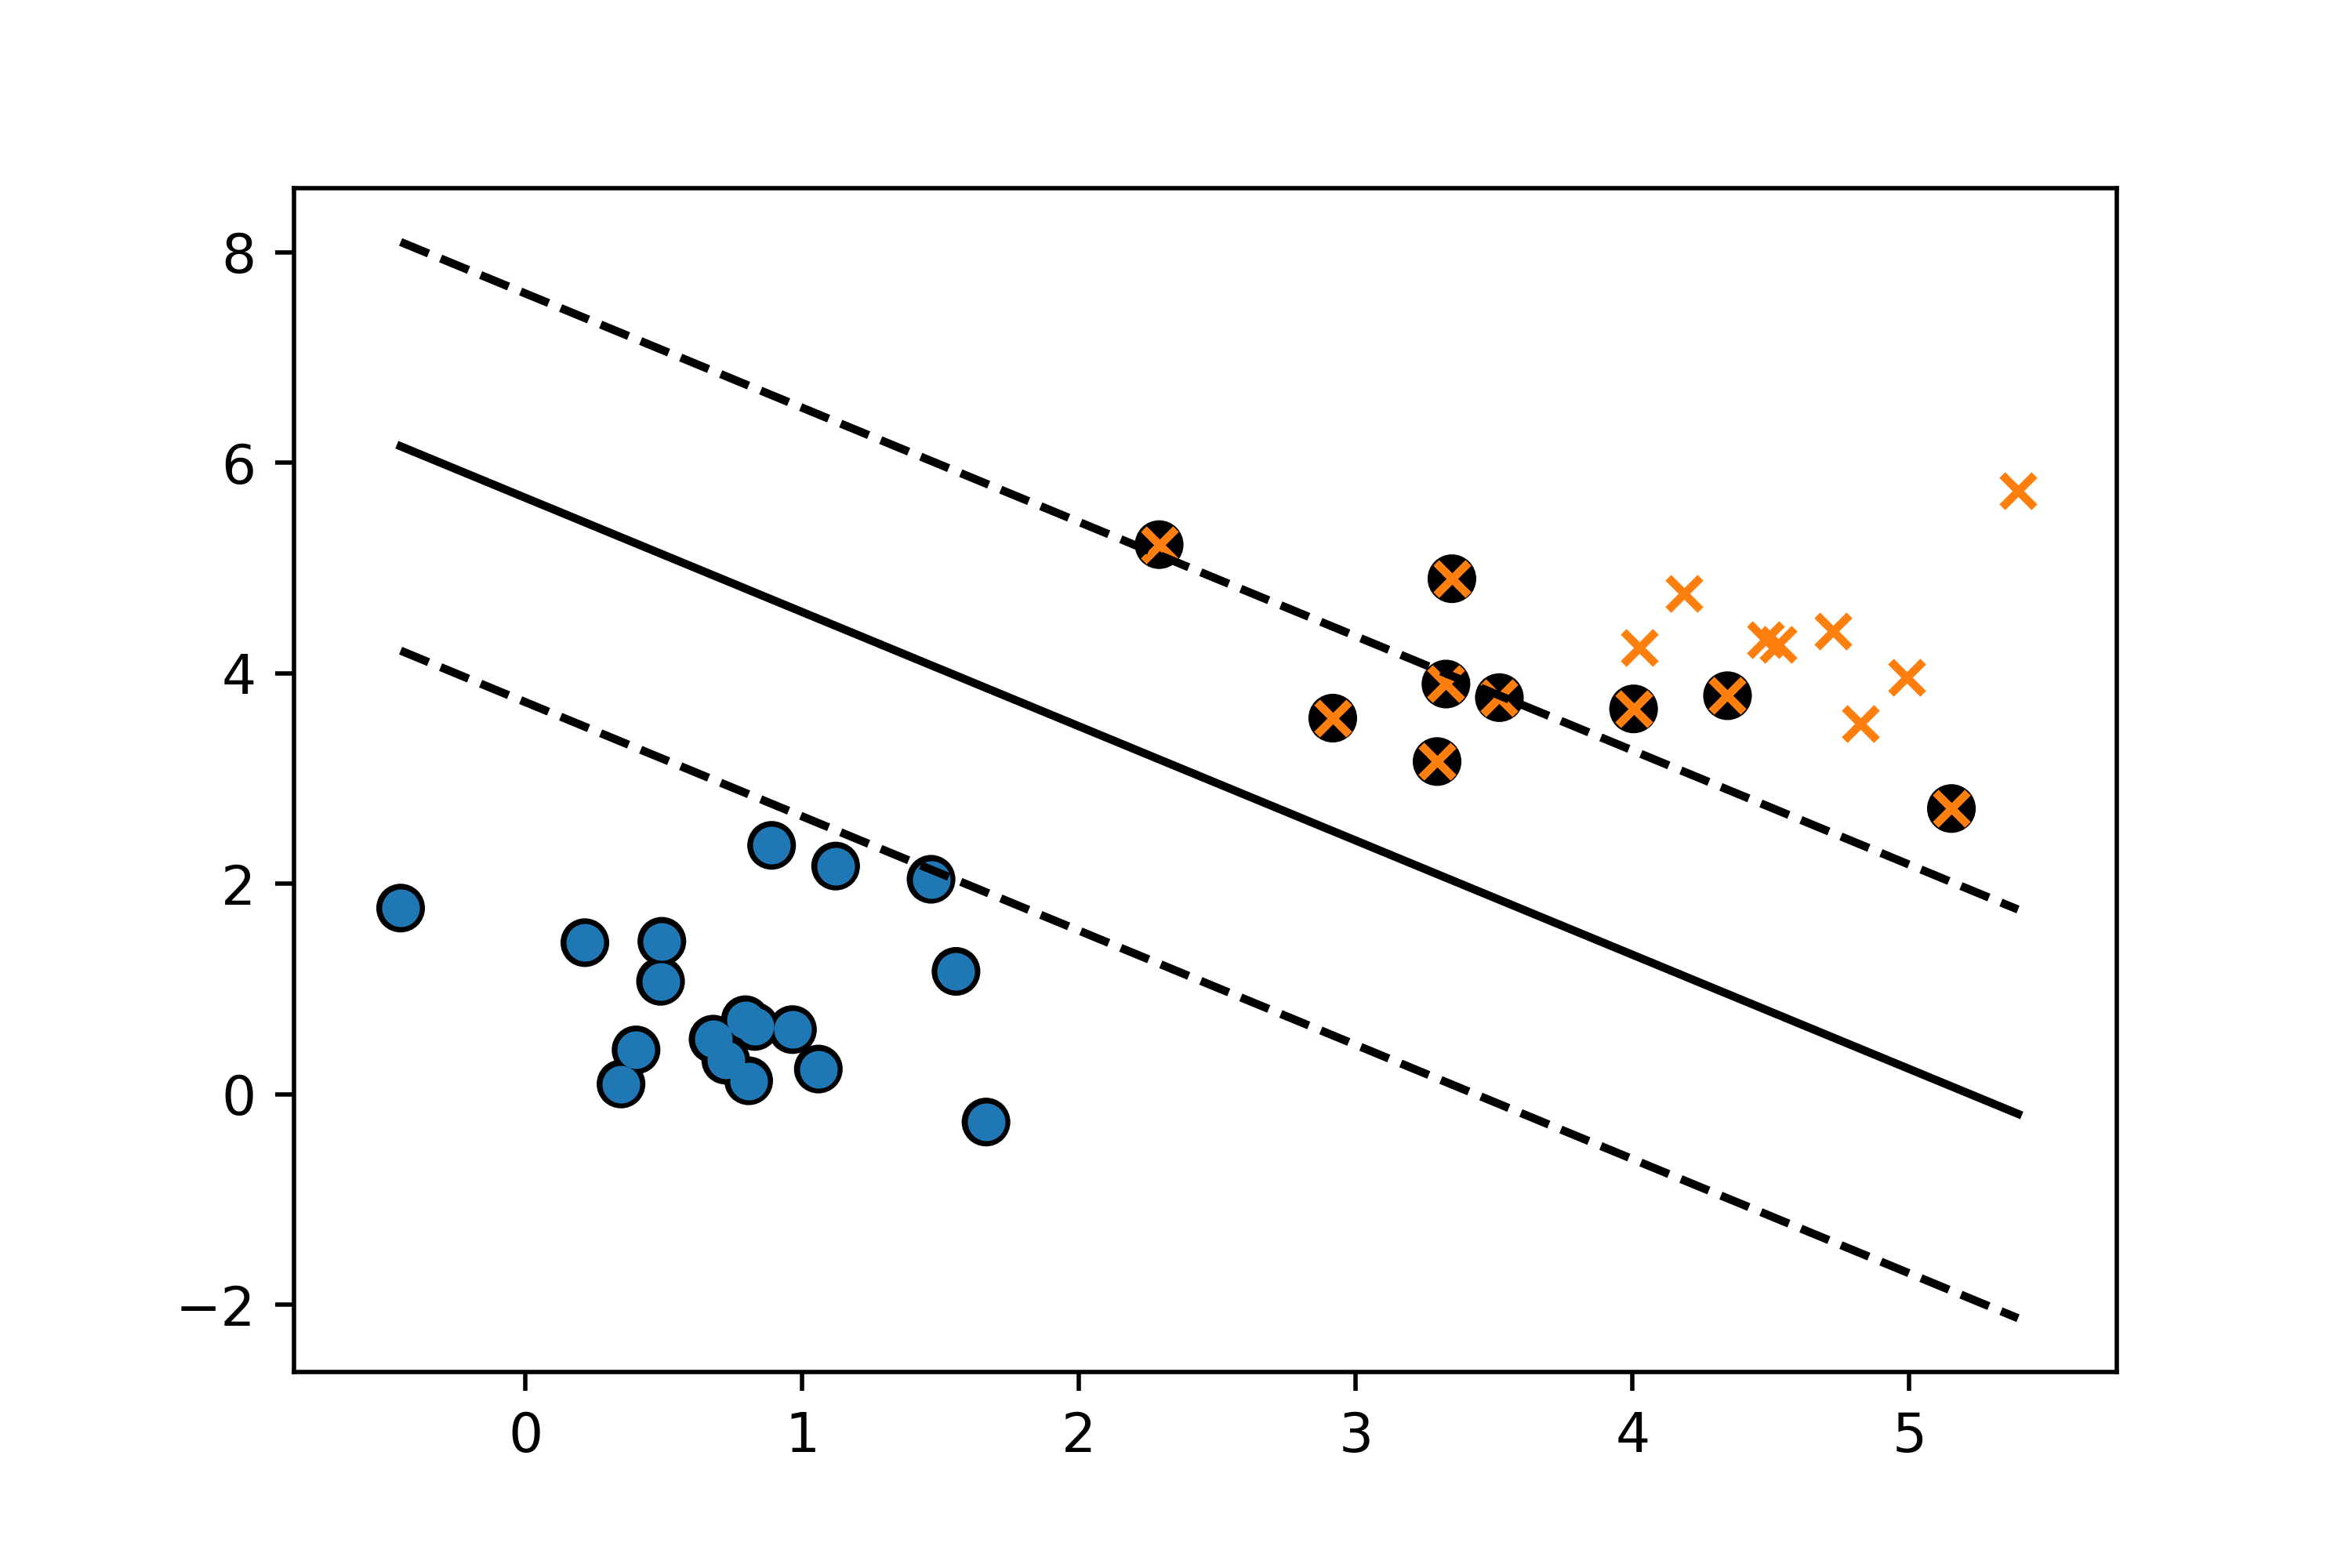
\includegraphics[scale=0.5]{SVM}
	\caption{مسئله حاشیه سخت در ماشین بردار پشتیبان}
	\label{fig:SVM}
\end{figure}

